\documentclass[12pt, a4paper]{article}

\usepackage[utf8]{inputenc}
\usepackage[spanish]{babel}
\usepackage{titling}
\usepackage[left=2cm,right=2cm,top=2cm,bottom=2cm]{geometry}
\usepackage{enumerate}
\usepackage{amsmath}
\usepackage{graphicx}
\usepackage{caption}
\usepackage{multicol}
\usepackage{float}

\usepackage{listings}%-para agregar codigo-
\usepackage[usenames,dvipsnames]{color}
\usepackage{color}%------------------------

%---------------------importar codigo desde archivos cpp----------------------------
\lstloadlanguages{C++}
\lstnewenvironment{code}
	{\csname lst@SetFirstLabel\endcsname}
	{\csname lst@SaveFirstLabel\endcsname}
% general command to set parameter(s)
\lstset{
	language=C++, basicstyle=\small\ttfamily, keywordstyle=\slshape,
	emph=[1]{tipo,usa}, emphstyle={[1]\sffamily\bfseries},
	morekeywords={tint,forn,forsn},
	basewidth={0.47em,0.40em},
	columns=fixed, fontadjust, resetmargins, xrightmargin=5pt, xleftmargin=15pt,
	flexiblecolumns=false, tabsize=2, breaklines, breakatwhitespace=false, extendedchars=true,
	numbers=left, numberstyle=\tiny, stepnumber=1, numbersep=9pt,
	frame=l, framesep=3pt,
	basicstyle=\ttfamily,
	keywordstyle=\color{blue}\ttfamily,
	stringstyle=\color{magenta}\ttfamily,
	commentstyle=\color{RedOrange}\ttfamily,
	morecomment=[l][\color{OliveGreen}]{\#}
}

\lstdefinestyle{C++}{
	language=C++, basicstyle=\small\ttfamily, keywordstyle=\slshape,
	emph=[1]{tipo,usa,tipo2}, emphstyle={[1]\sffamily\bfseries},
	morekeywords={tint,forn,forsn},
	basewidth={0.47em,0.40em},
	columns=fixed, fontadjust, resetmargins, xrightmargin=5pt, xleftmargin=15pt,
	flexiblecolumns=false, tabsize=2, breaklines,	breakatwhitespace=false, extendedchars=true,
	numbers=left, numberstyle=\tiny, stepnumber=1, numbersep=9pt,
	frame=l, framesep=3pt,
    basicstyle=\ttfamily,
    keywordstyle=\color{blue}\ttfamily,
    stringstyle=\color{magenta}\ttfamily,
    commentstyle=\color{RedOrange}\ttfamily,
    morecomment=[l][\color{OliveGreen}]{\#}
}

\def\nbtitle#1{\begin{Large}\begin{center}\textbf{#1}\end{center}\end{Large}}
\def\nbsection#1{\section{#1}}
\def\nbsubsection#1{\subsection{#1}}
\def\nbcoment#1{\begin{small}\textbf{#1}\end{small}}
\newcommand{\comb}[2]{\left( \begin{array}{c} #1 \\ #2 \end{array}\right)}
\def\complexity#1{\texorpdfstring{$\mathcal{O}(#1)$}{O(#1)}}
 \newcommand\cppfile[2][]{
\lstinputlisting[style=C++,linerange={#1}]{#2}
}
%------------------------------------------------------------------------------

\newcommand{\subtitulo}[1]{\begin{center}\textbf{#1}\end{center}}

\title{\textbf{Estructuras de datos}}
\author{Wilmer Emiro Castrillón Calderón}

% Para que busque los archivos en una carpeta arriba
\graphicspath{{../}}
\newcommand*\lstinputpath[1]{\lstset{inputpath=#1}}
\lstinputpath{../}
%------------------------------------------------------------------------------

\begin{document}
	\maketitle
	
	%<*Capitulo>
	
	\section{Tablas aditivas}
	Son estructuras de datos utilizadas para realizar operaciones acumuladas sobre un conjunto de datos estáticos 
	en un rango específico, es decir, ejecutar una misma operación(como por ejemplo la suma) sobre un intervalo 
	de datos, se asume que los datos en la estructura no van a cambiar. Estas estructuras también son conocidas como 
	\textit{Summed-area table} para el procesamiento de imágenes, a pesar de su nombre no necesariamente son 
	exclusivas para operaciones de suma, pues la idea general es aplicable a otras operaciones.\\
	
	Durante el cálculo de una misma operación sobre diferentes rangos se presenta superposición de problemas, las 
	tablas aditivas son utilizadas para reducir la complejidad computacional aprovechando estas superposiciones
	utilizando programación dinámica.
	
	\subtitulo{Ejemplo inicial.}
	
	Dado un vector V = \{5,2,8,2,4,3,1\} encontrar para múltiples consultas la suma de todos los elementos en un rango
	[i,j], indexando desde 1, por ejemplo con el rango [1, 3] la suma es [5+2+8] = 15.\\
	
	La solución trivial es hacer un ciclo recorriendo el vector entre el intervalo [i,j], en el peor de los casos se
	debe recorrer todo el vector, esto tiene una complejidad $O(n)$ puede que para una consulta sea aceptable, pero
	en casos grandes como por ejemplo un vector de tamaño $10^{5}$ y una cantidad igualmente grande de consultas el
	tiempo de ejecución se hace muy alto, por lo tanto se hace necesario encontrar una mejor solución.\\
	
	La operación suma tiene propiedades que nos pueden ayudar a resolver este problema de una forma mas eficiente:
	\begin{enumerate}[1.]
		\item La suma es asociativa es decir, se cumple: $a+(b+c)=(a+b)+c$, esto indica que sin importar 
			la agrupación que se realice el resultado sera igual (no confundir con propiedad conmutativa).
		\item La suma posee elemento neutro, es decir existe un $\beta$ tal que $a + \beta = a$, en la suma 
			$\beta = 0$.
		\item La suma tiene operación inversa, es decir existe una operación que puede revertir la suma, la cual 
			es la resta: si $a+b=c$ entonces $c-a=b$.
	\end{enumerate}
	
	Considerando las anteriores propiedades el problema se puede trabajar desde otro enfoque, primero se puede
	definir $suma(x)$ = $\sum_{k=1}^{x} V_{k}$, ahora tomando como ejemplo una consulta en el rango [3,5] 
	del vector $V$, se puede utilizar $suma(2) = V_{1}+V_{2}$ y $suma(5) = V_{1}+V_{2}+V_{3}+V_{4}+V_{5}$ para
	encontrar $V_{3}+V_{4}+V_{5}$, utilizando la propiedad asociativa se obtiene: 
	$(V_{1}+V_{2})+(V_{3}+V_{4}+V_{5})=(V_{1}+V_{2}+V_{3}+V_{4}+V_{5})$ y usando la propiedad inversa se llega a:
	$(V_{3}+V_{4}+V_{5})=(V_{1}+V_{2}+V_{3}+V_{4}+V_{5})-(V_{1}+V_{2})$ por lo tanto 
	$(V_{3}+V_{4}+V_{5})=suma(5)-suma(2)$. De esta manera el problema se puede generalizar como 
	$\sum_{k=i}^{j} V_{k} = suma(j) - suma(i-1)$ cuando $i \neq 1$ y $suma(j)$ cuando $i=1$.\\
	
	Ahora pre-calculando $suma(x)$ se puede dar una solución inmediata a cada consulta, esto se puede resolver 
	utilizando un enfoque básico de programación dinámica. Para encontrar $suma(x)$ se puede reescribir como: 
	$suma(x) = V_{x} + suma(x-1)$ con caso base $suma(1)=V_{1}$ y por definición la operación acumulada sobre un 
	conjunto vacío es igual al elemento neutro (esto significa que el indice cero tendrá el valor del elemento 
	neutro), a partir de esto se puede obtener la siguiente solución en C++ con consultas indexando desde 1.
	\cppfile[6-14]{Estructuras_de_datos/codigos/tablas_aditivas.cpp}
	
	De manera general las tablas aditivas son aplicables a cualquier operación que posea las tres propiedades 
	descritas anteriormente: ser asociativa, tener elemento neutro y operación inversa, por ejemplo la suma,
	multiplicación o el operador de bits XOR.

	\subtitulo{Tablas aditivas en 2D}
	
	Las operaciones acumuladas no solo se pueden usar sobre una dimension, sino también sobre n-dimensiones, en estos
	casos se debe trabajar con el principio de inclusión-exclusión pues se debe considerar mejor las operaciones entre
	intervalos, si no tiene en cuenta este principio las soluciones contendrían elementos duplicados o faltantes, lo 
	que produciría soluciones incorrectas.\\
	
	\textbf{Ejemplo:} dada la matriz $M$ encontrar para múltiples consultas la suma de todos los elemento en una
	submatriz $Q_{(i1,j1),(i2,j2)}$:
	\begin{center}
		$M = $
		\begin{tabular}{|l|l|l|l|l|}
			\hline
			1  &9  &6 &3 &7\\ \hline
			7  &5  &3 &0 &5\\ \hline
			0  &7  &6 &5 &3\\ \hline
			7  &8  &9 &5 &0\\ \hline
			9  &5  &3 &7 &8\\ \hline
		\end{tabular}
	\end{center}
	En el intervalo $Q_{(2,2),(3,4)}$ el resultado es $5+3+0+7+6+5=26$.\\

	En el caso de 1D se definió $suma(x)$ = $\sum_{k=1}^{x} V_{k}$, ahora esta debe tener dos dimensiones, es decir, 
	$suma(i,j)$ debe contener la suma de los elementos en la submatriz $Q_{(1,1),(i,j)}$, entonces ahora se definirá:
	$suma(i,j)$ = $\sum_{k=1}^{i} \sum_{w=1}^{j} M_{k,w}$, mas sin embargo pre-calcular $suma(i,j)$ de forma eficiente
	requiere de usar el principio de inclusión-exclusión, de manera trivial se puede calcular la primera fila como
	$suma(1,j)$ = $\sum_{w=1}^{j} M_{1,w}$ y la primera columna como $suma(i,1)$ = $\sum_{k=1}^{i} M_{k,1}$, en base
	a esto se puede calcular el resto de la matriz pero se debe tener algo de cuidado, por ejemplo si se toma 
	$suma(2,2) = suma(1,2) + suma(2,1) + M_{2,2}$ se obtendría un resultado incorrecto pues se estaría realizando la
	siguiente operación: $(M_{1,1}+M_{1,2}) + (M_{1,1},M_{2,1}) + M_{2,2}$, se puede observar que el elemento 
	$M_{1,1}$ se esta sumando dos veces, acá se aplica el principio de inclusión-exclusión: 
	$|A| \cup |B| = |A| + |B| - |A \cap B|$ lo que significa que hace falta quitar la intersección, esta es 
	$suma(1,1)$ entonce se puede generalizar como: $suma(i,j)$ = $M_{i,j} + suma(i-1,j) + suma(i,j-1) - suma(i-1,j-1)$
	cuando $i,j \neq 1$.\\
	
	Una vez construido el pre-calculo es necesario realizar las consultas, se utilizara como ejemplo la consulta en
	el rango $Q_{(2,2),(3,4)}$, de igual manera se debe tener cuidado de no sumar un mismo intervalo mas de una vez,
	entonces para encontrar la suma en este intervalo se tomaría $suma(i2,j2)$ esta contendría 
	$\sum_{k=1}^{i2} \sum_{w=1}^{j2} M_{k,w}$, esta tiene elemento adicionales como lo muestra la figura 
	\ref{estructuras:tablas_aditivas:img1}, al restarle $suma(i1-1,j2)$ se quitan algunos elementos 
	(figura \ref{estructuras:tablas_aditivas:img2}), al restarle $suma(i2,j1-1)$ pasaríamos a restar dos veces el intervalo 
	$M_{(1,1),(i1-1,j1-1)}$ (figura \ref{estructuras:tablas_aditivas:img3}), por lo tanto es necesario reponer lo faltante agregando
	$suma(i1-1,j1-1)$ (figura \ref{estructuras:tablas_aditivas:img4}), de esta manera se puede generalizar la formula: 
	$\sum_{k=i1}^{i2} \sum_{w=j1}^{j2} M_{k,w}$ = $suma(i2,j2)-suma(i1-1,j2)-suma(i2,j1-1)+suma(i1-1,j1-1)$.

	\begin{center}
		\begin{multicols}{4}
        	\begin{figure}[H]
        		\centering
				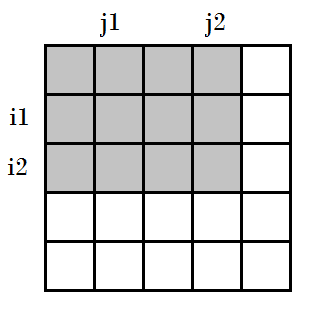
\includegraphics[scale=0.4]{Estructuras_de_datos/imagenes/tablas_aditivas/img1}
				\caption{}
				\label{estructuras:tablas_aditivas:img1}
			\end{figure}
			\columnbreak
			\begin{figure}[H]
				\centering
				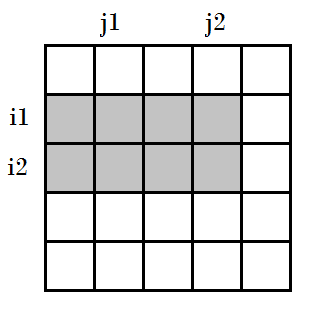
\includegraphics[scale=0.4]{Estructuras_de_datos/imagenes/tablas_aditivas/img2}
				\caption{}
				\label{estructuras:tablas_aditivas:img2}
			\end{figure}
			\columnbreak
			\begin{figure}[H]
				\centering
				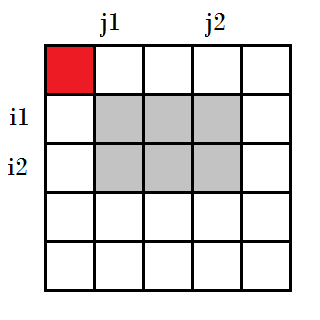
\includegraphics[scale=0.4]{Estructuras_de_datos/imagenes/tablas_aditivas/img3}
				\caption{}
				\label{estructuras:tablas_aditivas:img3}
			\end{figure}
			\columnbreak
			\begin{figure}[H]
				\centering
				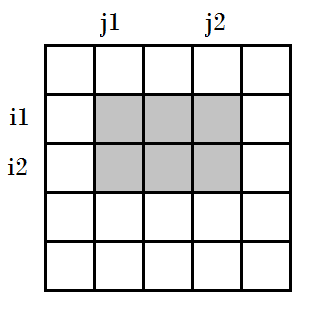
\includegraphics[scale=0.4]{Estructuras_de_datos/imagenes/tablas_aditivas/img4}
				\caption{}
				\label{estructuras:tablas_aditivas:img4}
			\end{figure}
    	\end{multicols}
	\end{center}
	
	Para la solución en C++ la fila y columna cero de la tabla donde se guardara el pre-calculo se deberá llenar
	con el elemento neutro, el cero, luego se debe llenar el resto de la tabla siguiendo las formulas antes 
	establecidas, este ejemplo es para consultas indexando desde 1.
	\cppfile[26-36]{Estructuras_de_datos/codigos/tablas_aditivas.cpp}
	
	\subtitulo{Tablas aditivas en 3D}
	
	Las tablas aditivas se pueden generalizar para trabajar en n-dimensiones, mas sin embargo la dificultad de hacer 
	los pre-cálculos y las consultas aumenta bastante, pues crece considerablemente la cantidad de operaciones a
	realizar. En el caso 3D igualmente se debe tener cuidado con el principio de inclusión-exclusión, el 
	pre-calculo se realizaría de la siguiente manera: sea 
	$suma(i,j,k)$ = $\sum_{x=1}^{i} \sum_{y=1}^{j} \sum_{z=1}^{k} V_{x,y,z}$, entonces  
	$suma(i,j,k) = V_{i,j,k} + suma(i,j,k-1)+suma(i-1,j,k)+suma(i,j-1,k)-suma(i-1,j-1,k)-suma(i-1,j,k-1)
	-suma(i,j-1,k-1)+suma(i-1,j-1,k-1)$, y para las consultas: $\sum_{x=i1}^{i2} \sum_{y=j1}^{j2} \sum_{z=k1}^{k2}
	V_{x,y,z} = suma(i2,j2,k2)-suma(i2,j2,k1-1)-suma(i1-1,j2,k2)+suma(i1-1,j2,k1-1)-suma(i2,j1-1,k2)
	+suma(i2,j1-1,k1-1)+suma(i1-1,j1-1,k2)-suma(i1-1,j1-1,k1-1)$.
	
	\subtitulo{Conclusiones}
	Esta estructura de datos facilita encontrar el valor acumulado de una operación sobre un rango de valores 
	estáticos, puede ser aplicada para operaciones que cumplan con las tres propiedades descritas
	anteriormente, la complejidad computacional de hacer el pre-calculo es lineal a la cantidad de
	elementos en la estructura, y las consultas se realizan en complejidad constante al realizar solamente operaciones
	directas sobre elementos en la tabla del pre-calculo. Si se requiere actualizar los valores de la tabla esto
	haría necesario actualizar el pre-calculo, esto representa que la operación de actualizar es lineal a la 
	cantidad de elementos, pero esa complejidad no suele ser favorable, por lo tanto se recomienda utilizar solo 
	en arreglos estáticos, y recurrir a otras estructuras como las Sparse table en el caso de arreglos dinámicos.
	
	\section{Disjoint set}
	Es una estructura de datos que permite agrupar elementos en conjuntos y consultar si dos elementos
	pertenecen a un mismo conjunto, contiene una estructura en forma de árbol pero con una implementacion poco
	compleja. La estructura consta de dos operaciones principales, $union(u, v)$ para unir los conjuntos que incluyen 
	a los nodos $u$ y $v$, y la operación $find(v)$ para indicar a cual conjunto pertenece un nodo $v$.\\
	
	Cada nodo tendrá la información de su nodo padre, y cada conjunto tiene un nodo raíz. Entonces se tiene un 
	arreglo lineal $p$ donde $p[v]$ tiene el padre del nodo $v$, para los nodos raíz se tendrá que $p[v]=v$, 
	como se muestra en la imagen siguiente, inicialmente cada nodo es un conjunto diferente entonces todo el arreglo 
	debe iniciar con $p[v]=v$.
	
	\begin{figure}[h!]
		\centering
		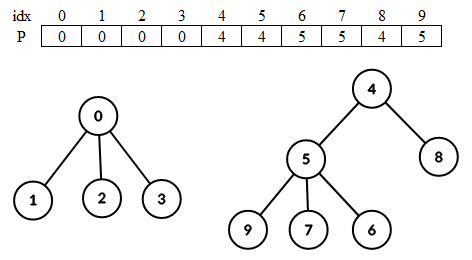
\includegraphics[scale=0.7]{Estructuras_de_datos/imagenes/disjoint_set/construccion}
		\caption{Disjoint set}
		\label{estructuras:disjoint_set:construccion}
	\end{figure}
	
	\subtitulo{Operación $Find$}
	
	La operación consiste en devolver el nodo raíz del conjunto al cual pertenece un nodo $v$, como cada nodo
	guarda el indice de su nodo padre, entonces solo se debe subir sobre el árbol hasta llegar al nodo raíz
	el cual se puede detectar con la condición $p[x]=x$.
	
	\subtitulo{Operación $Union$}
	
	Consiste en unir dos elementos $u$ y $v$ en un mismo conjunto, básicamente consiste en hacer que el nodo raíz 
	del conjunto de $u$ sea padre del nodo raíz del conjunto de $v$, de esta forma ambos nodos quedan dentro de un 
	mismo árbol, si $u$ y $v$ ya se encuentran dentro en un mismo conjunto entonces no se hace nada.

	\cppfile[7-27]{Estructuras_de_datos/codigos/disjoint_set_union_find.cpp}
	
	\subtitulo{Unión por rangos}
	
	Los disjoint set son estructuras flexibles que nos permiten realizar diferentes variantes para distintas tareas,
	una de ellas es la unión por rangos, la cual consiste en tener guardado en un arreglo la máxima
	profundidad que contiene cada nodo y nos permite durante la operación $Union$ unir el árbol de menor rango 
	a otro de mayor de rango. En la siguiente figura se observa un ejemplo de unir dos conjuntos con distinto rango,
	los conjuntos del nodo 9 y 8, sus raíces son 5 y 4 respectivamente, entonces como el nodo 4 tiene un rango mayor, 
	se volverá el padre del nodo 5.
	
	\begin{figure}[h!]
		\centering
		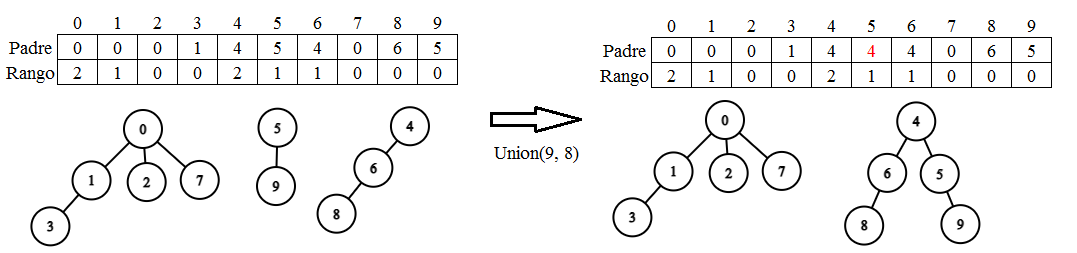
\includegraphics[scale=0.6]{Estructuras_de_datos/imagenes/disjoint_set/union_rango}
		\caption{Unión por rangos}
		\label{estructuras:disjoint_set:UnionRango}
	\end{figure}
	
	\cppfile[30-48]{Estructuras_de_datos/codigos/disjoint_set_union_find.cpp}
	
	\subtitulo{Compresión de caminos}
	
	Cuando se utiliza gran cantidad de nodos el disjoint set tradicional es ineficiente, debido a la posibilidad
	de formar arboles muy profundos, llevando a la operación $find(v)$ a tener complejidad $O(n)$ para cada 
	búsqueda, existe una optimización la cual permite reducir la profundidad de los arboles, de tal forma que la 
	máxima longitud de rangos sera 1, de esta forma se evita tener arboles profundos. La implementacion es sencilla
	y consiste que en cada búsqueda actualizar los nodos visitados como hijos directos del nodo raíz. La siguiente
	figura muestra como se vería el anterior ejemplo con compresión de caminos.
	
	\begin{figure}[!htb]
		\minipage{0.5\textwidth}
			\centering
			\includegraphics[scale=0.6]{Estructuras_de_datos/imagenes/disjoint_set/compresion}
			\caption{}
			\label{estructuras:disjoint_set:compresion}
		\endminipage
		\minipage{0.5\textwidth}
			\cppfile[16-21]{Estructuras_de_datos/codigos/union_find_compresion.cpp}
		\endminipage
	\end{figure}
	
	\subtitulo{Conclusiones}
	Esta estructura permite asociar elementos en conjuntos de forma eficiente, tiene múltiples aplicaciones como
	por ejemplo almacenar componentes conexas de grafos, es utilizada por otros algoritmos como el algoritmo de 
	kruskal para la búsqueda del árbol de expansión mínima en grafos, también se puede almacenar información
	adicional sobre los conjuntos como su cantidad de nodos o almacenar para cada nodo la lista de sus descendientes,
	entre otras aplicaciones.
	
	\section{Sparse table}
	
	Es una estructura de datos para realizar operaciones sobre rangos en un conjunto datos lineales, esta 
	estructura utiliza un precálculo sobre los valores iniciales para poder realizar consultas en complejidad 
	logarítmica, permite realizar operaciones que cumplen con la propiedad asociativa como la suma o la función 
	mínimo(el valor mínimo entre dos valores), una de sus ventajas es su implementación corta, sin embargo esta 
	estructura no permite actualizaciones, por lo que debe ser usada con datos estáticos.\\
	
	Esta estructura aprovecha la propiedad de que todo número entero se puede representar de forma única como 
	sumas de potencias de dos, consiste en operar rangos del arreglo que tengan longitudes de potencia de dos y 
	guardarlos en una tabla de precálculo, se utiliza una matriz de $n$ filas y $log_{2}(n)$ columnas, la primera 
	columna contendrá el arreglo inicial, las demás columnas tendrán la operación acumulada en el rango 
	$[i, i+2^{j})$ del arreglo inicial, para cada consulta se operan los valores de sólo algunos rangos, evitando que 
	se operen todos los valores en el intervalo. Para la explicación de construcción y consulta se usará un vector 
	$V$ para los valores iniciales, una matriz $SP$ para guardar el sparse table y la operación suma.\\
	
	La construcción es corta y consiste de inicialmente llenar la primera columna con los valores iniciales 
	$SP_{i,0} = V_{i}$, y para las demás columnas se aplica la siguiente fórmula 
	$SP_{i,j} = SP_{i,j-1} + SP_{i+2^{j-1},j-1}$, con $1 \leq j \leq log_{2}(n)$ y $1 \leq i+2^{j}-1 < n$, al 
	final cada posición de la matriz tendrá los siguientes valores $SP_{i,j} = \sum_{x=i}^{i+2^{j}-1} V_{x}$ con
	$0 \leq i < n$ y $0 \leq i+2^{j}-1 < n$. La construcción tiene una complejidad $O(n*log_{2}(n))$.
	
	\begin{figure}[!htb]
		\minipage{0.5\textwidth}
			\centering
			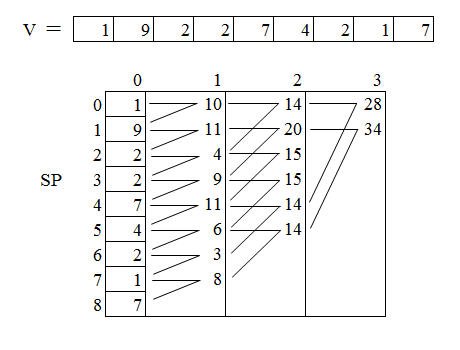
\includegraphics[scale=0.65]{Estructuras_de_datos/imagenes/sparse_table/construccion}
			\caption{}
			\label{estructuras:sparse_table:construccion}
		\endminipage
		\minipage{0.5\textwidth}
			\cppfile[9-17]{Estructuras_de_datos/codigos/sparse_table.cpp}
		\endminipage
	\end{figure}
	
	Para las consultas se debe tener en cuenta que $SP_{i,j}$ guarda la operación acumulada en el intervalo 
	$[i,i+2^{j}-1]$, Entonces para obtener la operación acumulada en un rango 
	$[L,R]$ se debe tomar la fila $L$ y buscar el máximo $j$ tal que $L+2^{j}-1 \leq R$ es decir, tomar el intervalo 
	mas grande que no se salga del rango $[L,R]$, con esto ya se tiene el acumulado de una parte del intervalo, de tal 
	forma que se puede actualizar el rango a $[L+2^{j}, R]$ y repetir el proceso hasta encontrar el valor de todo el
	intervalo $[L,R]$; la complejidad es $O(log_{2}(n))$. Por ejemplo para calcular suma en el rango $[1,6]$ se puede 
	obtener con solo sumar dos valores 
	de la tabla, el primero $SP_{1,2}$ el cual contiene la suma en el rango [1,4] y el segundo $SP_{5,1}$ el cual
	contiene la suma en el rango $[5,6]$, entonces resultado es $26$, como se muestra en la figura 
	\ref{estructuras:sparse_table:consulta}.
	
	\begin{figure}[!htb]
		\minipage{0.5\textwidth}
			\centering
			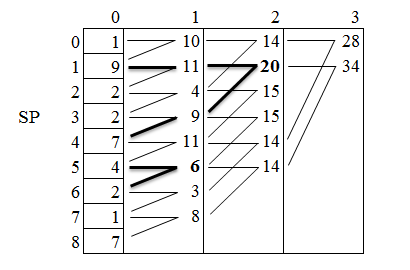
\includegraphics[scale=0.65]{Estructuras_de_datos/imagenes/sparse_table/consulta}
			\caption{}
			\label{estructuras:sparse_table:consulta}
		\endminipage
		\minipage{0.5\textwidth}
			\cppfile[19-27]{Estructuras_de_datos/codigos/sparse_table.cpp}
		\endminipage
	\end{figure}
	
	\subtitulo{Optimización para operaciones idempotentes}
	
	Las operaciones idempotentes son aquellas que se pueden aplicar múltiples veces y el resultado será el mismo que 
	al aplicarse la primera vez, es decir $f(f(x))=f(x)$, por ejemplo las funciones mínimo y máximo, para este tipo 
	de casos se puede trabajar con intervalos superpuestos y la respuesta seguirá siendo igual, por ejemplo para 
	encontrar el RMQ en un intervalo $[L,R]$ con $L < R$ se cumple que $RMQ(L,R) = min(RMQ(L,R-1), RMQ(L+1,R))$, 
	entonces la consulta sobre el sparse table se puede simplificar para este tipo de funciones, de tal forma que 
	solo dos intervalos son suficientes para encontrar la respuesta acumulada en cualquier rango, estos intervalos 
	serán $[L,L+2^j]$ y $[R-2^j+1,R]$ con $j = floor(log_{2}(R-L+1))$ de esta forma la complejidad es $O(1)$.
	\cppfile[29-32]{Estructuras_de_datos/codigos/sparse_table.cpp}

	
	%\section{Bibliografia}
	
	%https://en.wikipedia.org/wiki/Summed-area_table.\\ 
	%http://trainingcamp.org.ar/anteriores/2017/clases.shtml.\\ 
	%libro: competitive programming 3.\\ 

	%</Capitulo>
	
\end{document}



